\documentclass[10pt]{article}
\usepackage[margin=1in, paperwidth=8.5in, paperheight=11in]{geometry}
\usepackage{ifpdf,amsmath, amssymb, comment, color, graphicx, stmaryrd,setspace,enumitem,tikz, fancyhdr, wrapfig, textcomp, units, mathptmx, pdfpages, cancel, multicol}
\usepackage{hyperref}
\hypersetup{
    colorlinks=true,
    urlcolor=blue,
}

\setlength{\headheight}{14.5pt}
\newcommand{\Q}{\mathbb{Q}}
\newcommand{\R}{\mathbb{R}}
\newcommand{\Z}{\mathbb{Z}}
\newcommand{\vu}{\mathbf{u}}
\newcommand{\vv}{\mathbf{v}}
\newcommand{\vw}{\mathbf{w}}
\newcommand{\vi}{\mathbf{i}}
\newcommand{\vj}{\mathbf{j}}
\newcommand{\vk}{\mathbf{k}}
\newcommand{\vn}{\mathbf{n}}
\newcommand{\vr}{\mathbf{r}}
\newcommand{\va}{\mathbf{a}}
\newcommand{\vF}{\mathbf{F}}
\newcommand{\vL}{\mathbf{L}}
\newcommand{\vT}{\mathbf{T}}
\newcommand{\vN}{\mathbf{N}}
\newcommand{\proj}{\operatorname{proj}}
\newcommand{\orth}{\operatorname{orth}}
\newcommand\del\nabla
\newcommand\dotp[1][.5]{\,\mathbin{\vcenter{\hbox{\scalebox{#1}{$\bullet$}}}}\,}

% Solution text is in red. If you want the solutions to show, remove the \iffalse from the definition of the \red command.
%\newcommand{\red}[1]{ %\iffalse
%	\textcolor{red}{#1} }%\fi}

\newenvironment{red}{\color{red}}{\ignorespacesafterend}
\newcommand{\blue}[1]{\textcolor{blue}{#1}}
\newcommand{\green}[1]{\textcolor{green}{#1}}
\renewcommand{\section}[1]{\begin{center} \textbf{#1} \\\end{center}}
%
\hyphenpenalty=5000
\setlength{\parindent}{0in}
%\oddsidemargin=-.25in
\allowdisplaybreaks
\pagestyle{fancy}
\renewcommand{\headrulewidth}{0pt}
\lhead{MATH 202}
\rhead{Spring 2022}
%\lfoot{\copyright\ CLEAR Calculus 2010}
\cfoot{}

\begin{document}
%


%\onehalfspacing
\allowdisplaybreaks
%##################################################################
\section{PS\#1: Numerical integration - \red{Answer key} }

\begin{red}
(Note: I split the derivative review questions off into their own separate pdf.)
\end{red}

\begin{enumerate}[leftmargin=0pt]

\item[2.] In class on Wednesday, we computed exact values for \(\displaystyle\int_0^1(1-x^2)\, dx\) and \(\displaystyle\int_1^2 \frac{1}{x^2}\, dx\). Show your work using the \href{https://activecalculus.org/single/sec-4-4-FTC.html}{Fundamental Theorem of Calculus} to compute these values. No decimal approximations, please!
\begin{red}
\begin{align*}
    \int_0^1(1-x^2)\,dx &= \left[x - \frac13 x^3\right|_0^1 \\
    &= \left(1 - \frac13\cdot 1^3\right) - \left(0 - \frac13\cdot  0^3\right) = 1 - \frac13 = \frac23 \\
    \int_1^2 \frac{1}{x^2}\, dx &= \int_1^2 x^{-2}\, dx \\
    &= \left[\frac{1}{-1}\cdot x^{-1}\right|_1^2 
    = \left[\frac{-1}{x}\right|_1^2 \\
    &= \left(\frac{-1}{2}\right) - \left(\frac{-1}{1}\right) = -\frac{1}{2} + 1 = \frac{1}{2}
\end{align*}
\end{red}
    
\item[3.] The width $w_n$, in feet, at various points $x_n$ along the fairway of a golf course changes as shown in the figure below. The values of $w_n$ and $x_n$ are given in the table below the figure.

\begin{center}
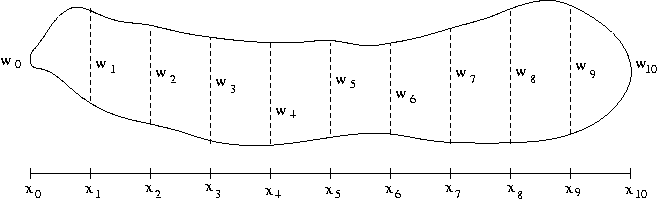
\includegraphics[width=.75\textwidth]{images/webwork-fertilizer.png}
\end{center}

\[\begin{array}{|l|l|l|l|l|l|l|l|l|l|l|l|}
\hline
n=    & 0 & 1  & 2   & 3   & 4   & 5   & 6   & 7   & 8   & 9   & 10  \\ \hline
x_n= & 0 & 90 & 180 & 270 & 360 & 450 & 540 & 630 & 720 & 810 & 900 \\ \hline
w_n= & 0 & 70 & 78  & 83  & 85  & 77  & 72  & 74  & 79  & 79  & 0   \\ \hline
\end{array}\]
If one pound of fertilizer covers 225 square feet, find a reasonable estimate for the amount of fertilizer needed to fertilize the fairway.

\begin{red}
(\textbf{NOTE}: Your numbers may vary from the ones presented here, because Webwork generates numbers randomly. I think the solution method will still be comprehensible, no matter what numbers you have.)

Overall, the strategy is to compute the area of each little slice of the fairway by multiplying $w_n$ by $\Delta x$, add all the areas together (hence this is some kind of Riemann sum), and then divide by the coverage-per-pound number. 

A left Riemann sum would use $w_0$ through $w_9$, and a right Riemann sum would use $w_1$ through $w_{10}$. Since $w_0$ and $w_{10}$ are both $0$, these values will end up being the same. (So the trapezoid estimate will also be the same, since it's the average of the left and the right Riemann sums.) I'll write out the left sum for illustration:

\begin{align*}
    \textrm{Area} &\approx 90\cdot (w_0 + w_1 + \cdots + w_9) \\
    &= 90\cdot(0+70+78+83+85+77+72+74+79+79) = 62730\textrm{ sq ft} \\
   \textrm{Fertilizer} &\approx \frac{62730 \textrm{ sq ft}}{225\textrm{ sq ft / lb}} \approx 278.8 \textrm{ lb}
\end{align*}
\end{red}


\end{enumerate}
\end{document}